\documentclass[final]{proposal}
\usepackage[utf8]{vietnam}
\usepackage{placeins}
\usepackage{amsfonts}
\usepackage{textcomp}
\usepackage{dblfloatfix}
\usepackage{lineno}
\usepackage{amssymb}
\usepackage{tabularx,booktabs}
\usepackage{longtable, lipsum}
\usepackage{amsmath}
\usepackage{mathtools}
\usepackage{graphicx}
\usepackage{lscape}
\usepackage{caption}
\usepackage{hyperref}
\usepackage[sorting=nyt]{biblatex}
\usepackage{mathtools}
\usepackage{lipsum}
\usepackage{fancyhdr}
\usepackage{titlesec}
\usepackage{makecell}
\usepackage{listings}
\usepackage{subcaption}
\usepackage{adjustbox}
\usepackage[vietnamese,english]{babel}
\usepackage{multirow}
\usepackage{longtable}
\usepackage{rotating}
\usepackage{chngcntr}
% Define color and column type
\definecolor{dkgreen}{rgb}{0,0.6,0}
\definecolor{gray}{rgb}{0.5,0.5,0.5}
\definecolor{mauve}{rgb}{0.58,0,0.82}
\newcolumntype{C}[1]{>{\centering\arraybackslash}m{#1}}

% Config reference source file
\addbibresource{references/section2.bib}
\addbibresource{references/section3.bib}

% Config figure path
\graphicspath{ {./graphics} }

% Config for math in quantum computin
\DeclarePairedDelimiter\bra{\langle}{\rvert}
\DeclarePairedDelimiter\ket{\lvert}{\rangle}
\DeclarePairedDelimiterX\braket[2]{\langle}{\rangle}{#1 \delimsize\vert#2}

% Config listings 
\lstset{
  frame=tb,
  aboveskip=3mm,
  belowskip=3mm,
  showstringspaces=false,
  columns=fullflexible,
  basicstyle={\small\ttfamily},
  numbers=left,
  numberstyle=\tiny\color{gray},
  keywordstyle=\color{blue},
  commentstyle=\color{dkgreen},
  stringstyle=\color{mauve},
  breaklines=true,
  postbreak=\mbox{\textcolor{red}{$\hookrightarrow$}\space},
  tabsize=3
}
% Config listings 
\lstset{
  frame=tb,
  aboveskip=3mm,
  belowskip=3mm,
  showstringspaces=false,
  columns=fullflexible,
  basicstyle={\small\ttfamily},
  numbers=left,
  numberstyle=\tiny\color{gray},
  keywordstyle=\color{blue},
  commentstyle=\color{dkgreen},
  stringstyle=\color{mauve},
  breaklines=true,
  postbreak=\mbox{\textcolor{red}{$\hookrightarrow$}\space},
  tabsize=3
}

% Config information thesis
% =========== Thay đổi thông tin tại phần này ===========
\upperuniname{ĐẠI HỌC QUỐC GIA THÀNH PHỐ HỒ CHÍ MINH}
\uniname{TRƯỜNG ĐẠI HỌC CÔNG NGHỆ THÔNG TIN}
\title{Đánh giá hiệu năng và tính mở rộng của hệ thống Hadoop Distributed File System}
\titleen{Evaluating the Performance and Scalability of the Hadoop Distributed File System}
\supervisorname{TS. LÊ DUY TÂN }
\stuname{NGUYỄN HỒNG SƠN }
\proposaltype{Môn chuyên đề nghiên cứu 3}
% =========== Hết phần thay đổi thông tin ===========

% Begin thesis
\begin{document}


\headerbox
\vnproposalheader
\proposalname

% Begin main thesis, start page numbering
\mainmatter
\counterwithin{equation}{section}
\counterwithin{table}{section}
\counterwithin{figure}{section}
\setcounter{secnumdepth}{3}



% \section{Tóm tắt}

Trong giai đoạn hiện nay, nhu cầu dữ liệu cho học máy cũng như các lĩnh vực khác liên tục tăng lên, do đó hệ thống lưu trữ chúng phải thích ứng với nhu cầu ngày càng tăng về hiệu suất, độ tin cậy và khả năng chịu lỗi. Điều này làm tăng độ phức tạp quản trị và chi phí. Cải thiện hiệu suất và tăng khả năng mở rộng của hệ thống trong khi vẫn duy trì chi phí thấp là rất quan trọng. Các giải pháp phần mềm lưu trữ được cho là hướng đi mới do giải pháp phần cứng vẫn quá đắt đỏ. 

Hadoop Distributes File System (HDFS) do  Apache Software Foundation phát triển đến nay đã có phiên bản thứ 3, là một giải pháp đáng tin cậy để lưu trữ và phân phối dữ liệu một cách đáng tin cậy trên nhiều node. Nghiên cứu này xem xét cách HDFS hoạt động trong thiết lập với các phần mềm hỗ trợ phân quyền và bảo mật khác như Kerberos, Openldap, Apache Ranger, YARN. Nghiên cứu thay đổi số lượng các node lưu trữ và tính toán để kiểm tra khả năng mở rộng của hệ thống. Nghiên cứu hướng đến việc thử nghiệm và kiểm tra tính chính xác các cam kết của HDFS, đồng thời phát hiện các điểm có tiềm năng cải tiến. Nghiên cứu này sẽ cải thiện hiểu biết về vệ thống HDFS cho cộng đồng, đồng thời thông qua các kịch bản được trình bày để giải quyết các hạn chế về hiệu suất của HDFS.
\pagestyle{fancy}
\fancyhf{}
\fancyfoot[C]{\thepage}
\if @twoside
  \fancyhead[EL,OR]{\bfseries\nouppercase\rightmark}
\else
  \fancyhead[R]{\bfseries\nouppercase\rightmark}
\fi


\section{Introduction}

\lipsum

\subsection{Subsection 1}
\lipsum
\lipsum
\subsubsection{subsubsection 1}
\lipsum
\lipsum
\section{Giới thiệu}

Sự ra đời của Big Data và Machine Learning đã thúc đẩy nhiều nhà khoa học và các tập đoàn tập trung sang phát triển lĩnh vực này, khiến nhu cầu về lưu trữ dữ liệu tăng nhanh. Do đó, các giải pháp quản lý và lưu trữ dữ liệu mới được phát triển. Trong nghiên cứu này, tác giả giới thiệu và thực sự một số đánh giá hiệu năng của HDFS\cite{borthakur2007hadoop}, một phần mềm cung cấp hệ thống lưu trữ phân tán được thiết kế với khả năng dễ mở rộng, có hiệu quả cao, khả năng chịu lỗi tốt, đồng thời có chi phí triển khai thấp. 

Sự phức tạp của hệ phân tán nói chung và HDFS nói riêng đòi hỏi các cấu hình và điều chỉnh cẩn thận để đạt hiệu suất tốt, các thay đổi được thực hiện ảnh hưởng tới toàn hệ thống và có khả năng làm mất mát dữ liệu nếu không được thao tác đúng. Các dữ liệu lưu trong hệ thống hầu hết đều là dữ liệu nhạy cảm như: dữ liệu thô, dữ liệu sau xử lý, dữ liệu huấn luyện và các mô hình sản sinh. Việc quản lý truy cập, vừa thuận tiện cho người sử dụng, đồng thời đảm bảo các tiêu chí của an toàn dữ liệu là rất quan trọng. Kết hợp các công cụ quản lý xác thực và định danh mã nguồn mở đã được kiểm chứng như  OpenLDAP \cite{openLdap}, Kerberos \cite{bellovin1990limitations}, Apache Ranger \cite{ApacheRanger} sẽ khắc phục được những nhược điểm của HDFS.

Bên cạnh đó, do mức độ lớn và quan trọng của dữ liệu, nó chịu áp lực độ chịu lỗi đối với sự hao mòn không thể tránh khỏi của phần cứng, cũng chịu áp lực về hiệu suất khi áp dụng các phương thức xác thực và mã hóa dữ liệu. Tìm hiểu và đánh giá hiệu suất toàn diện của hệ thống là cần thiết. Trong nghiên cứu này, tác giả xây dựng và trả lời các câu hỏi sẽ giúp đáp ứng một số nhu cầu lưu trữ dữ liệu phân tán lớn, yêu cầu khả năng chịu lỗi cao, thuận tiện trong phân quyền và đồng thời tốc độ truy cập nhanh. Khả năng tích hợp với các ứng dụng khác cũng được khảo sát và đề xuất. Trong trường hợp nào thì hệ thống hoạt động tốt nhất? Nếu như vậy thì cái giá phải đánh đổi là gì? Hệ thống hoạt động thế nào khi dữ liệu tăng lên cao hoặc nhiều người dùng cùng truy cập? Khi xảy ra hư hỏng phần cứng thì ứng dụng sẽ điều hướng lưu trữ như thế nào? Các giải pháp theo dõi hiệu suất hệ thống khả dụng là gì? Khi nào thì hiệu suất của hệ thống giảm?

Phần còn lại của nghiên cứu được trình bày như sau: Phần \ref{section3-background} trình bày các thành phần cơ bản của HDFS và các nghiên cứu liên quan. Phần \ref{section4-method} trình bày thiết kế hệ thống và khác thực nghiệm. Phần \ref{section4-experiment} trình bày chi tiết các kết quả. Cuối cùng, kết luận và đề xuất được trình bày ở phần \ref{section5-conclusion}.
\section{Cơ sở lý thuyết và các nghiên cứu liên quan}
\label{section3-background}

\lipsum
\lipsum
\lipsum
\section{Phân tích thiết kế hệ thống}
\label{section4-method}

\section{Thực nghiệm và kết quả}
\label{section4-experiment}

Phần này, trình bày một số kết quả dự kiến của đề tài khi hoàn thành.

\begin{itemize}
    \item Một hệ thống hadoop sẵn sàng để phục vụ storage, có quản lý truy cập dựa trên role-base access control. Công cụ quản lý thuận lợi, thực hiện bằng ứng dụng web như ví dụ tại các hình \ref{fig:sec5-ranger-portal}, \ref{fig:sec5-hadoop-portal}, \ref{fig:sec5-yarn-portal}
    \item Dữ liệu đánh giá hệ thống 
\end{itemize}

\begin{figure}
    \centering
    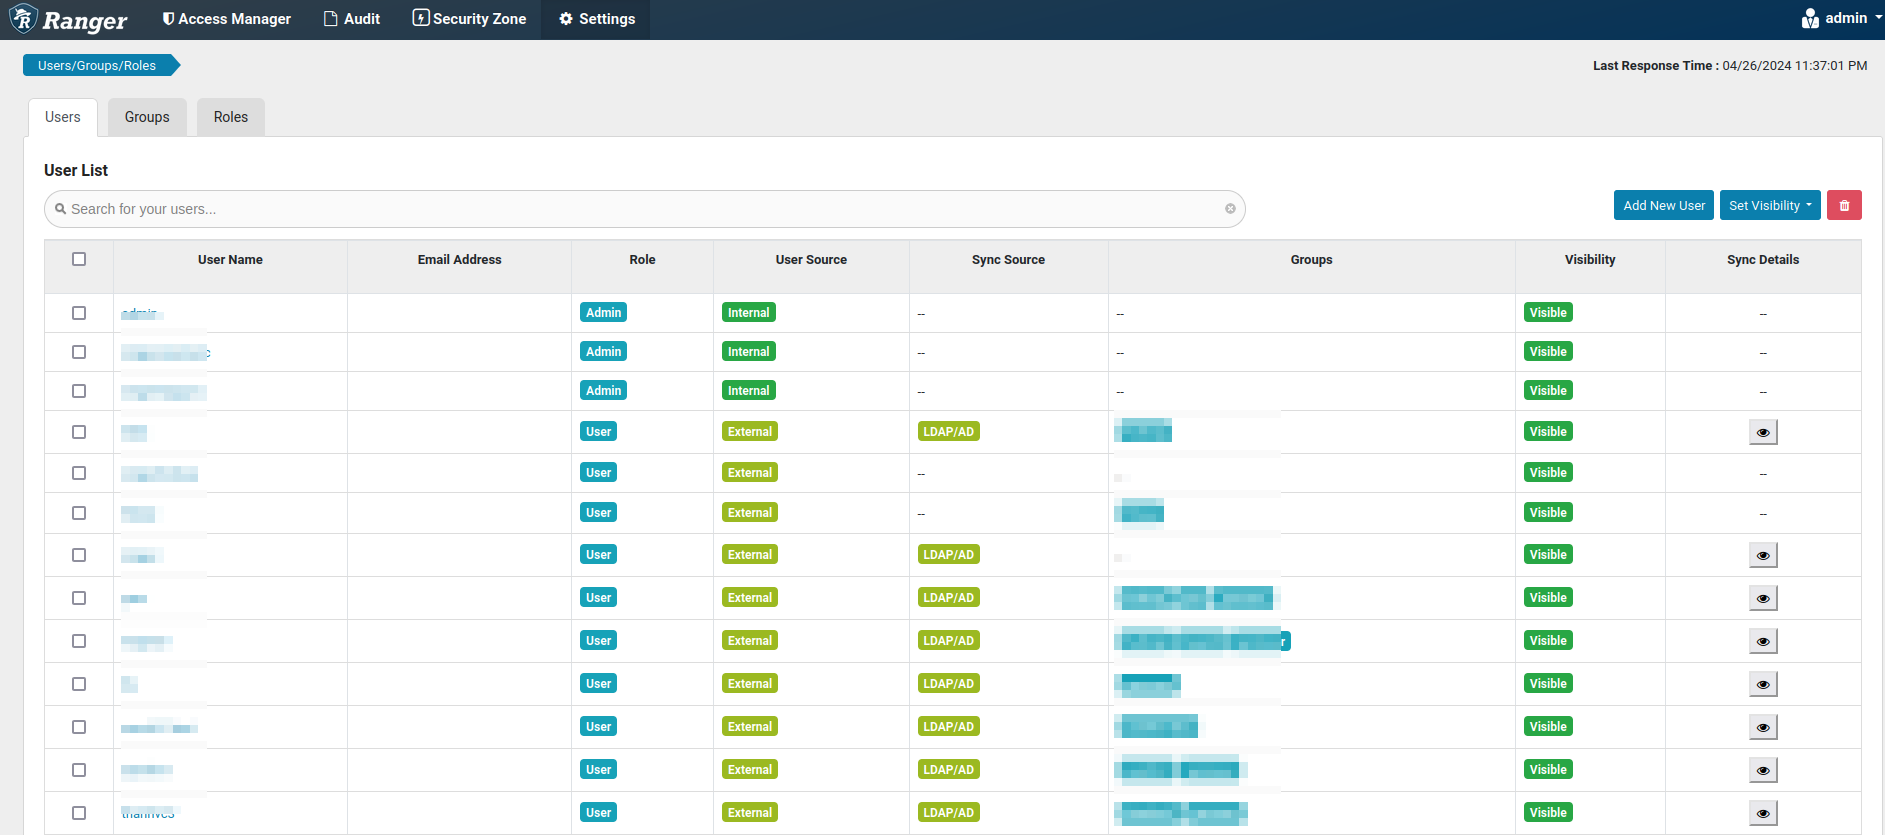
\includegraphics[scale=0.3]{section5/sec5-ranger-portal.png}
    \caption{Dự kiến giao diện quản lý người dùng trên Ranger}
    \label{fig:sec5-ranger-portal}
\end{figure}

\begin{figure}
    \centering
    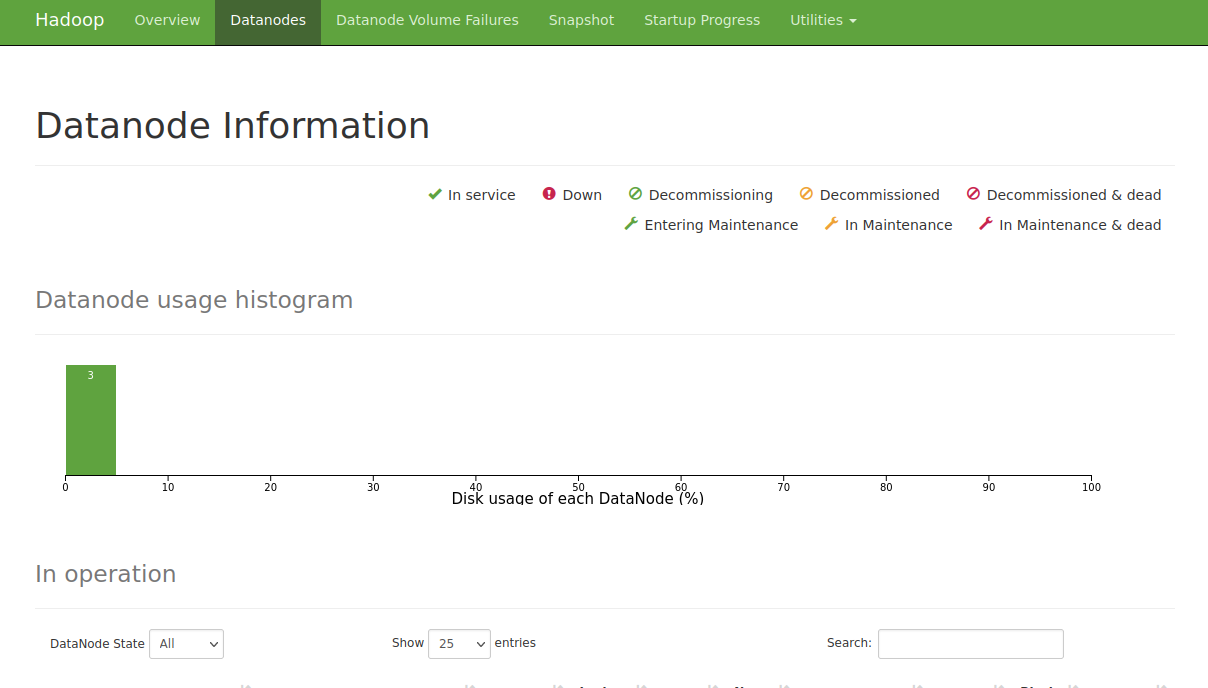
\includegraphics[scale=0.3]{section5/sec5-hadoop-portal.png}
    \caption{Dự kiến giao diện hadoop cluster}
    \label{fig:sec5-hadoop-portal}
\end{figure}

\begin{figure}
    \centering
    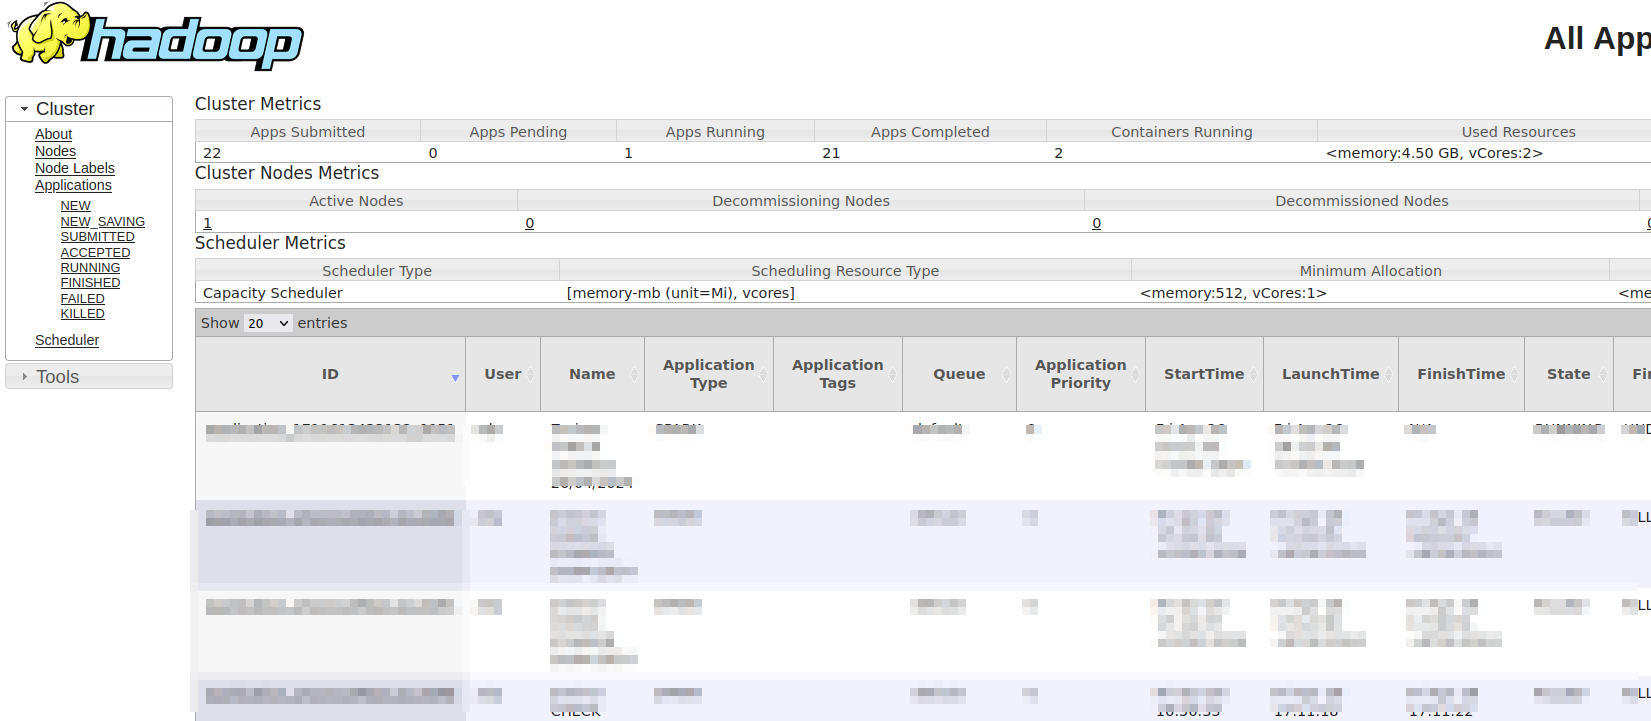
\includegraphics[scale=0.3]{section5/sec5-yarn-portal.png}
    \caption{Dự kiến giao diện yarn cluster}
    \label{fig:sec5-yarn-portal}
\end{figure}
\section{Kết luận và phương hướng}
\label{section6-conclusion}

\lipsum
\lipsum
\lipsum
\newpage
\tableofcontents
\printbibliography[heading=bibintoc, title = {Tài liệu tham khảo}]
\end{document}
